% Figure 1 from Yitian Chen, Agent Based Modeling for Group Alignment.
% Source: agent-based-modelling/paper.tex in the supplied repository.
\begin{figure}[ht]
    \centering
    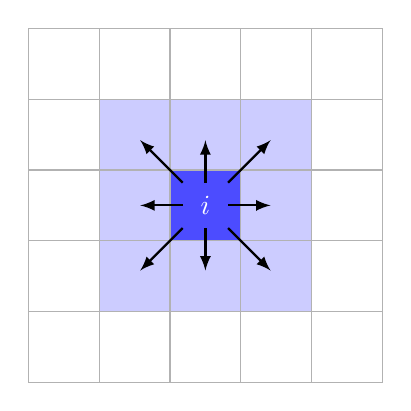
\begin{tikzpicture}[scale=0.9]
        % 5x5 background grid
        \foreach \x in {0,...,4}
            \foreach \y in {0,...,4}
                \draw[gray!50] (\x,\y) rectangle ++(1,1);
        % Moore neighbourhood
        \foreach \x in {1,2,3}
            \foreach \y in {1,2,3}
                \fill[blue!20] (\x,\y) rectangle ++(1,1);
        % centre agent
        \fill[blue!70] (2,2) rectangle ++(1,1);
        \node[white] at (2.5,2.5) {$i$};
        % redraw borders on top
        \foreach \x in {0,...,4}
            \foreach \y in {0,...,4}
                \draw[gray!60] (\x,\y) rectangle ++(1,1);
        % arrows to the 8 neighbours
        \foreach \dx/\dy in {1/0,-1/0,0/1,0/-1,1/1,1/-1,-1/1,-1/-1}
            \draw[-latex,thick] ({2.5+0.32*\dx},{2.5+0.32*\dy}) -- ({2.5+0.92*\dx},{2.5+0.92*\dy});
    \end{tikzpicture}
    \caption{Moore neighbourhood: agent $i$ propagates to its $k=8$ surrounding cells (shaded).}
    \label{fig:moore-neighbourhood}
\end{figure}
